%%%%%%%%%%%%%%%%%%%%%%%%%%%%%%%%%%%%%%%%%%%%%%%%%%%
%
%  New template code for TAMU Theses and Dissertations starting Fall 2016.  
%
%
%  Author: Sean Zachary Roberson
%  Version 3.17.09
%  Last Updated: 9/21/2017
%
%%%%%%%%%%%%%%%%%%%%%%%%%%%%%%%%%%%%%%%%%%%%%%%%%%%
%%%%%%%%%%%%%%%%%%%%%%%%%%%%%%%%%%%%%%%%%%%%%%%%%%%%%%%%%%%%%%%%%%%%%%
%%                           SECTION III
%%%%%%%%%%%%%%%%%%%%%%%%%%%%%%%%%%%%%%%%%%%%%%%%%%%%%%%%%%%%%%%%%%%%%

\chapter{RESULTS}
The radio altimeter tests described in this work were developed over a two year long process which can be approximately separated into three distinct phases of testing.  

\section{General Plotting Scripts}
This setup shows introduces the two general types of plots used across all tests, called `Height Plots' and `Stat Plots' respectively. The form of these was evolved over the course of different testing regimens to communicate the results from each effectively, but the basic plots introduce a standard format in which results from an altimeter test are displayed. 
\subsection{Height Plots}
\subsection{Stat Plots}

\section{Initial Testing Regimen}\label{sec:initial_results}

\section{Expanded In Band Tests}\label{sec:dvsg_ib_results}
\section{Out of Band Testing}\label{sec:dvsg_oob_results}
Another table is placed here to show the effect of having tables in multiple sections. The list of tables should still double space between table titles, while single spacing long table titles.

%Fix table labeling.
%\begin{table}[h!]
%	\centering
%	\begin{tabular}{|l|l|}
%		\hline
%		Dates & Attendance  \\ \hline
%		August 8-10, 2008 & 3,523  \\ \hline
%		August 14-16, 2009 & 4,003 \\ \hline
%		July 9-11, 2010 & 5,049 \\ \hline
%		August 5-7, 2011 & 6,891  \\ \hline
%		August 10-12, 2012 & 9,464  \\ \hline
%		August 16-18, 2013 & 11,077  \\ \hline
%		July 18-20, 2014 & 14,686 \\ \hline
%		July 31-August 2, 2015 & 18,411  \\ \hline
%	\end{tabular}
%	\caption{San Japan attendance. Data is taken from \cite{ANCONS}. I intentionally make the title of this table long so the single space effect is seen in the list of tables.}
%\end{table}
%
%You may be wondering why San Japan was chosen. There are a few reasons as to why I did this:
%
%\begin{enumerate}
%\item It is one of the fastest-growing anime conventions in Texas.
%\item Filler.
%\item I wanted a good variety of table examples.
%\item Because conventions are cool.
%\end{enumerate}
%
%The \textit{enumerate} environment was used to generated an ordered list above.
%
%\section{Section Test Example}
%We insert another figure here, just for kicks.
%
%\begin{figure}[h!]
%	\centering
%	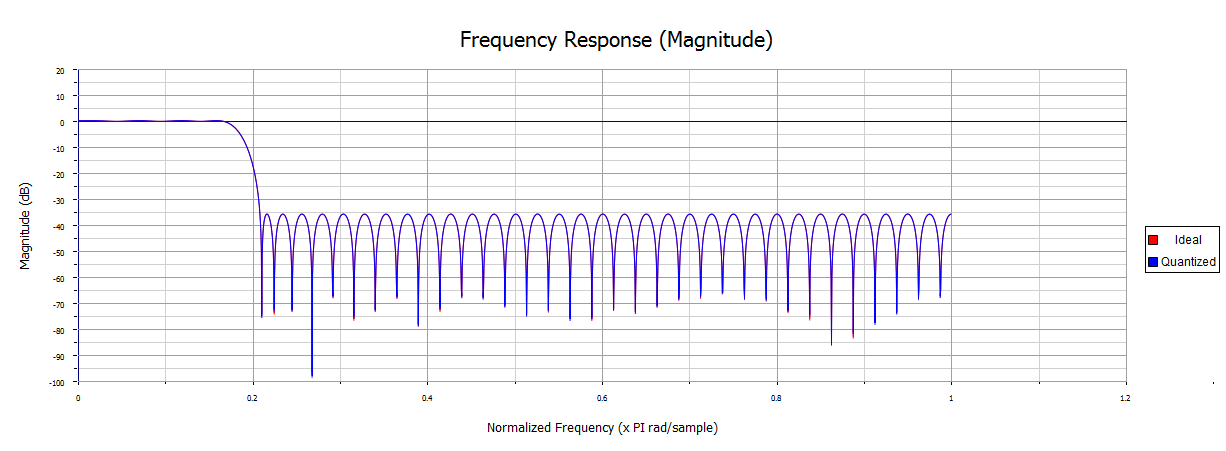
\includegraphics[width = 6.0in]{LowPass_Filter_Design.png}
%	\caption{A low pass filter design.}
%\end{figure}
